\subsection{CONTINUOUS FUNCTIONS}

DEFINITION 1. A mapping \(f\) of a topological space \(\mathbf{X}\) into a topological space \(\mathbf{X}'\) is said to be continuous at a point \(x_0 \in \mathbf{X}\) if, given any neighbourhood \(\mathbf{V}'\) of \(f(x_0)\) in \(\mathbf{X}'\) , there is a neighbourhood \(\mathbf{V}\) of \(x_0\) in \(\mathbf{X}\) such that the relation \(x \in \mathbf{V}\) implies \(f(x) \in \mathbf{V}'\) .

Definition 1 may be restated in the following more intuitive form: to say that \(f\) is continuous at the point \(x_0\) means that \(f(x)\) is as near as we please to \(f(x_0)\) whenever \(x\) is sufficiently near \(x_0\) .

The relation ``for each \(x \in V\) , \(f(x) \in V'\) '' is equivalent to \(f(V) \subset V'\) or again to \(V \subset \overline{f}^{1}(V')\) ; in view of the neighbourhood axiom \((V_{I})\) , we see that Definition 1 is equivalent to the following: \(f: X \to X'\) is said to be continuous at the point \(x_{0}\) if, for each neighbourhood \(V'\) of \(f(x_{0})\) in \(X'\) , \(\overline{f}^{1}(V')\) is a neighbourhood of \(x_{0}\) in X. Moreover, it is sufficient that \(\overline{f}^{1}(V')\) is a neighbourhood of \(x_{0}\) for each neighbourhood \(V'\) belonging to a fundamental system of neighbourhoods of \(f(x_{0})\) in \(X'\) (§ 1, no. 3).

PROPOSITION 1. Let \(f\) be a mapping of a topological space \(\mathbf{X}\) into a topological space \(\mathbf{X}'\) . If \(f\) is continuous at \(x\) , and if \(x\) lies in the closure of a subset \(A\) of \(X\) , then \(f(x)\) lies in the closure of \(f(A)\) .

Let \(\mathbf{V}'\) be a neighbourhood of \(f(x)\) in \(\mathbf{X}'\) . Since \(f\) is continuous at \(x\) , \(\overline{f}^1 (\mathbf{V}')\) is a neighbourhood of \(x\) in \(\mathbf{X}\) . Hence \(\overline{f}^1 (\mathbf{V}')\) meets \(\mathbf{A}\) , from which it follows that \(\mathbf{V}'\) meets \(f(\mathbf{A})\) , and therefore \(f(x)\) is in the closure of \(f(\mathbf{A})\) .

PROPOSITION 2. Let X, X', X'' be three topological spaces; let f be a mapping of X into X', continuous at x ∈ X; let g be a mapping of X' into X'', continuous at f(x). Then the composition h = g \(\circ\) f: X → X'' is continuous at x.

Let \(V''\) be a neighbourhood of \(h(x) = g(f(x))\) in \(X''\) . Since \(g\) is continuous at \(f(x)\) it follows that \(\overline{g}^1(V'')\) is a neighbourhood of \(f(x)\) in \(X'\) . But \(f\) is continuous at \(x\) , hence \(\overline{f}^1(\overline{g}^1(V'')) = \overline{h}^1(V'')\) is a neighbourhood of \(x\) in \(X\) , and therefore \(h\) is continuous at \(x\) .

DEFINITION 2. A mapping of a topological space X into a topological space X' is said to be continuous on X (or just continuous) if it is continuous at each point of X.

Examples. 1) The identity mapping of a topological space X onto itself is continuous.

\begin{enumerate}
\def\labelenumi{\arabic{enumi})}
\setcounter{enumi}{1}
\item
  A constant map of a topological space into a topological space is continuous.
\item
  Every mapping of a discrete space into a topological space is continuous.
\end{enumerate}

THEOREM 1. Let \(f\) be a mapping of a topological space \(X\) into a topological space \(X'\) . Then the following statements are equivalent:

\begin{enumerate}
\def\labelenumi{\alph{enumi})}
\item
  \(f\) is continuous in \(\mathbf{X}\) .
\item
  For every subset A of X, \(f(\overline{\mathrm{A}}) \subset \overline{f(\mathrm{A})}\) .
\item
  The inverse image under \(f\) of every closed subset of \(\mathbf{X}'\) is a closed subset of \(\mathbf{X}\) .
\item
  The inverse image under \(f\) of every open subset of \(\mathbf{X}'\) is an open subset of \(\mathbf{X}\) .
\end{enumerate}

We have already seen that a) implies b) (Proposition 1). To show that b) implies c), let \(\mathbf{F}'\) be a closed subset of \(\mathbf{X}'\) and let \(\mathbf{F} = \overline{f}^{1}(\mathbf{F}')\) ; then by hypothesis \(f(\overline{\mathbf{F}}) \subset \overline{f(\mathbf{F})} \subset \overline{\mathbf{F}}' = \mathbf{F}'\) , hence \(\overline{\mathbf{F}} \subset \overline{f}^{1}(\mathbf{F}') = \mathbf{F} \subset \overline{\mathbf{F}}\) , so that \(\mathbf{F} = \overline{\mathbf{F}}\) and \(\mathbf{F}\) is closed. By virtue of the relation \(\complement \overline{f}^{1}(A') = \overline{f}^{1}(\complement A')\) for every subset \(A'\) of \(X'\) , c) implies d). Finally, suppose that d) is satisfied. Let \(x\) be any point of \(X\) and let \(V'\) be any neighbourhood of \(f(x)\) in \(X'\) ; then there is an open set \(A'\) in \(X'\) for which

\[
f (x) \in \mathrm{A} ^ {\prime} \subset \mathrm{V} ^ {\prime}
\]

and hence \(x \in \overline{f}^1(\mathbf{A}') \subset \overline{f}^1(\mathbf{V}')\) . By hypothesis, \(\overline{f}^1(\mathbf{A}')\) is open in \(\mathbf{X}\) , so that \(\overline{f}^1(\mathbf{V}')\) is a neighbourhood of \(x\) in \(\mathbf{X}\) . Thus d) implies a).

Remarks. 1) Let \(\mathfrak{B}\) be a base (§ 1, no. 3) of the topology of \(\mathbf{X}'\) ; then for \(f: \mathbf{X} \to \mathbf{X}'\) to be continuous, it is necessary and sufficient that \(\overline{f}^1(\mathbf{U}')\) is open in \(\mathbf{X}\) for every \(\mathbf{U}' \in \mathfrak{B}\) .

Examples. Let \(a\) be any rational number. The mapping \(x \to a + x\) of the rational line \(\mathbf{Q}\) into itself is continuous on \(\mathbf{Q}\) , for the inverse image under this mapping of an open interval \(]b, c[\) is the open interval

\[
] b - a, c - a [.
\]

Likewise, the mapping \(x \to ax\) is continuous on \(\mathbf{Q}\) ; this is clear if \(a = 0\) , for then \(ax = 0\) for all \(x\) ; if \(a \neq 0\) then the inverse image under this mapping of the open interval \(]b, c[\) is the open interval with end-points \(b / a\) and \(c / a\) .

\pandocbounded{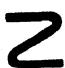
\includegraphics[keepaspectratio]{images/part001_4077020d.jpg}}

\begin{enumerate}
\def\labelenumi{\arabic{enumi})}
\setcounter{enumi}{1}
\tightlist
\item
  The direct image of an open (resp. closed) set of X under a continuous mapping \(f: \mathbf{X} \to \mathbf{X}'\) is not necessarily open (resp. closed) in \(\mathbf{X}'\) (cf.~§ 5).
\end{enumerate}

Example. * The mapping \(f: x \to 1 / (1 + x^2)\) of \(\mathbf{R}\) into itself is continuous, but \(f(\mathbf{R})\) is the half-open interval {[}0, 1{]}, which is neither open nor closed in \(\mathbf{R}\) . *

THEOREM 2. 1) If \(f: \mathbf{X} \to \mathbf{X}'\) and \(g: \mathbf{X}' \to \mathbf{X}''\) are two continuous mappings, then \(g \circ f: \mathbf{X} \to \mathbf{X}''\) is continuous.

\begin{enumerate}
\def\labelenumi{\arabic{enumi})}
\setcounter{enumi}{1}
\tightlist
\item
  For a bijection \(f\) of a topological space \(X\) onto a topological space \(X'\) to be a homeomorphism, it is necessary and sufficient that \(f\) and the inverse of \(f\) are continuous (or, as is also said, that \(f\) is bicontinuous).
\end{enumerate}

The first assertion is an immediate consequence of Proposition 2; the second follows from Theorem 1, d) and the definition of a homeomorphism (§ 1, no. 1).

\pandocbounded{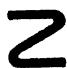
\includegraphics[keepaspectratio]{images/part001_720050f1.jpg}}

Remarks. 1) It is possible to have a continuous bijection of a topological space X onto a topological space X' which is not bicontinuous: for example, take X' to be the rational line Q, and X to be the set Q with the discrete topology; then the identity map X → X' is continuous but is not a homeomorphism.

\begin{enumerate}
\def\labelenumi{\arabic{enumi})}
\setcounter{enumi}{1}
\item
  To verify that a continuous bijection \(f: \mathbf{X} \to \mathbf{X}'\) is a homeomorphism, it is enough to show that for each \(x \in \mathbf{X}\) and each neighbourhood \(V\) of \(x\) , \(f(V)\) is a neighbourhood of \(f(x)\) in \(\mathbf{X}'\) .
\item
  Let X be a topological space, and for each \(x \in X\) let \(\mathfrak{B}(x)\) be the set of all neighbourhoods of x. Let \(x_{0}\) be a point of X; for each \(x \in X\) , define a set \(\mathfrak{B}_{0}(x)\) of subsets of X as follows: \(\mathfrak{B}_{0}(x_{0}) = \mathfrak{B}(x_{0})\) , and if \(x \neq x_{0}\) then \(\mathfrak{B}_{0}(x)\) is to be the set of all subsets of X which contain x. It is immediately verified (§ 1, no. 2, Proposition 2) that the sets \(\mathfrak{B}_{0}(x)\) are sets of neighbourhoods of points of X for a topology on X; let \(X_{0}\) denote the topological space thus obtained, and let \(j : X_{0} \to X\) denote the identity map, which is continuous but not in general bicontinuous. A mapping f of X into a topological space \(X'\) is continuous at the point \(x_{0}\) if and only if the composition \(X_{0} \stackrel{j}{\to} X \stackrel{f}{\to} X'\) is continuous on \(X_{0}\) ; this follows immediately from the definitions.
\end{enumerate}

